\documentclass{article}

%% PAQUETES

% Paquetes generales
\usepackage[margin=2cm, paperwidth=210mm, paperheight=297mm]{geometry}
\usepackage[spanish]{babel}
\usepackage[utf8]{inputenc}
\usepackage{gensymb}

% Paquetes para estilos
\usepackage{textcomp}
\usepackage{setspace}
\usepackage{colortbl}
\usepackage{color}
\usepackage{color}
\usepackage{upquote}
\usepackage{xcolor}
\usepackage{listings}
\usepackage{caption}
\usepackage[T1]{fontenc}
\usepackage[scaled]{beramono}

% Paquetes extras
\usepackage{amssymb}
\usepackage{float}
\usepackage{graphicx}
\usepackage{url}

%% Fin PAQUETES


% Definición de preferencias para la impresión de código fuente.
%% Colores
\definecolor{gray99}{gray}{.99}
\definecolor{gray95}{gray}{.95}
\definecolor{gray75}{gray}{.75}
\definecolor{gray50}{gray}{.50}
\definecolor{keywords_blue}{rgb}{0.13,0.13,1}
\definecolor{comments_green}{rgb}{0,0.5,0}
\definecolor{strings_red}{rgb}{0.9,0,0}

%% Caja de código
\DeclareCaptionFont{white}{\color{white}}
\DeclareCaptionFont{style_labelfont}{\color{black}\textbf}
\DeclareCaptionFont{style_textfont}{\it\color{black}}
\DeclareCaptionFormat{listing}{\colorbox{gray95}{\parbox{16.78cm}{#1#2#3}}}
\captionsetup[lstlisting]{format=listing,labelfont=style_labelfont,textfont=style_textfont}

\lstset{
	aboveskip = {1.5\baselineskip},
	backgroundcolor = \color{gray99},
	basicstyle = \ttfamily\footnotesize,
	breakatwhitespace = true,   
	breaklines = true,
	captionpos = t,
	columns = fixed,
	commentstyle = \color{comments_green},
	escapeinside = {\%*}{*)}, 
	extendedchars = true,
	frame = lines,
	keywordstyle = \color{keywords_blue}\bfseries,
	language = Oz,                       
	numbers = left,
	numbersep = 5pt,
	numberstyle = \tiny\ttfamily\color{gray50},
	prebreak = \raisebox{0ex}[0ex][0ex]{\ensuremath{\hookleftarrow}},
	rulecolor = \color{gray75},
	showspaces = false,
	showstringspaces = false, 
	showtabs = false,
	stepnumber = 1,
	stringstyle = \color{strings_red},                                    
	tabsize = 2,
	title = \null, % Default value: title=\lstname
	upquote = true,                  
}

%% FIGURAS
\captionsetup[figure]{labelfont=bf,textfont=it}
%% TABLAS
\captionsetup[table]{labelfont=bf,textfont=it}

% COMANDOS

%% Titulo de las cajas de código
\renewcommand{\lstlistingname}{Código}
%% Titulo de las figuras
\renewcommand{\figurename}{Figura}
%% Titulo de las tablas
\renewcommand{\tablename}{Tabla}
%% Referencia a los códigos
\newcommand{\refcode}[1]{\textit{Código \ref{#1}}}
%% Referencia a las imagenes
\newcommand{\refimage}[1]{\textit{Imagen \ref{#1}}}


\begin{document}
\pagenumbering{roman}
\setcounter{page}{5}

% TÍTULO, AUTORES Y FECHA
\begin{titlepage}
	\vspace*{\fill}
	\begin{center}
		\Large 75.06 Organización de Datos \\
		\Huge TP N°1: Catálogo discográfico \\
		\bigskip\huge\textit{Grupo 07} \\
		\bigskip\bigskip\bigskip\bigskip\bigskip\bigskip
		\bigskip\bigskip\bigskip\bigskip\bigskip\bigskip\bigskip
		\medskip\huge\textit{``Documentación de diseño''} \\
		\date{}
	\end{center}
	\vspace*{\fill}
\end{titlepage}
\newpage



% ÍNDICE
\tableofcontents
\newpage
\pagenumbering{arabic}


% INTRODUCCIÓN
\section{Introducción}
	
	El siguiente documento tiene como objetivo especificar y precisar los detalles técnicos de la realización de la primera parte del trabajo práctico. Se explican los problemas surgidos a la hora del diseño y las soluciones encaradas para solventar los mismos.
	\par
	Todos los archivos y códigos fuente aquí mencionados y relacionados al proyecto, así como también el presente informe, pueden ser encontrados y descargados del repositorio del grupo (\url{https://github.com/federicomrossi/7506-tp-grupo07}).
\bigskip




% REQUERIMIENTOS PLANTEADOS
\section{Requerimientos planteados}

	El trabajo solicitado se basa en la creación de un sistema para la generación de un catalogo a partir de archivos de letras de canciones de diversos autores. Dicho sistema debe ser capaz de realizar búsquedas por autor, titulo y frases, entregando como resultado los temas que coincidan con los parámetros ingresados.
	\par
	A su vez se exigieron ciertas condiciones para la realización del trabajo a la hora del manejo de las estructuras. El índice para la búsqueda por titulo debía estructurarse como un hash, por autor como un árbol B+ y los archivos de texto como bloques de registros variables.
	\par
	El producto final es una aplicación de consola que permite realizar las operaciones pedidas.
	\bigskip




% DIVISION DEL TRABAJO
\section{División del trabajo}

	El trabajo esta divido en tres capas funcionales: la física, la lógica y el front-end.
	\par
	A su vez, la capa lógica esta formada por tres módulos principales, a saber, el árbol B+, el hash extensible y las estructuras de recuperación de textos. La distribución mencionada se puede observar en la \textit{Figura 1}.
	\bigskip\medskip


% Figura 1
\begin{figure}[h]
	\centering
	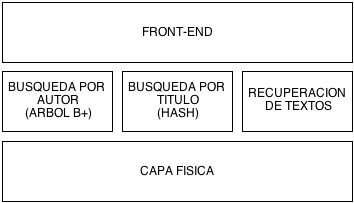
\includegraphics[width=0.48\textwidth]{images/DivisionModulos.png}
	\medskip
	\caption{Esquema de la estructuración en capas.}
\end{figure}
\bigskip\smallskip


	Esta división esta fundamentada en tener el menor acoplamiento posible entre las clases y sobretodo entre los módulos lógicos. A su vez, permite una fácil división de las tareas entre los integrantes del grupo de trabajo.
	\medskip




% DETALLES TECNICOS
\section{Detalles técnicos}

	A continuación se describirá con un mayor nivel de detalle cada una de los módulos que componen el sistema.
\smallskip


% DETALLES TECNICOS - Capa Física
\subsection{Capa Física}
	
	La capa física de este trabajo se centra alrededor de dos clases: \textit{ArchivoBloques} y \textit{SerialBuffer}.
	\par	
	La primera es la encargada de la interacción directa con el disco. La misma define interfaces para poder leer y escribir un archivo en función de bloques de un tamaño fijo y parametrizable.
	\par
	El problema que surgió aquí es que independientemente de utilizar el modo normal de apertura para escribir de C++ (ios::out), el archivo era truncado y se perdía su contenido, quedando solamente el último bloque escrito. La solución para esto fue que si se quería modificar un bloque ya existente, se utilizara un archivo de trabajo temporal para pasar el contenido original, intercalar el bloque a modificar y luego copiar el resto del archivo. Posteriormente se elimina el archivo original y se renombra el de trabajo. Debido a que esto es muy costoso y generalmente muchas de las operaciones de escritura consisten en agregar un nuevo bloque al final, existe un método que abre el archivo en modo append (ios::app) y agrega el nuevo bloque. La lectura en cambio no presento problema alguno.
	\par
	SerialBuffer es la clase encargada de brindar los medios para poder persistir de manera ordenada los registros de cada estructura. La misma presenta dos métodos principales, pack y unpack.
	\par
	El primero se encarga de agregar registros a un buffer de caracteres (cabe aclarar que se escogió por archivos de tipo binario para la persistencia de datos). Para poder recuperar la información a posteriori, antes de empaquetar cada registro carga en el buffer un prefijo de longitud para poder saber cuanto va a tener que recuperar del buffer a un objeto.
	\par
	El segundo, hace el trabajo inverso y restaura la información de un buffer, que previamente se leyó desde el disco, a un objeto. Utiliza el prefijo de longitu para saber la cantidad de caracteres a pasar desde el buffer al objeto de destino.
	\par
	Como puede notarse, el buffer es la estructura fundamental y puede verse al mismo como una sucesión de registros como la siguiente:
	\bigskip


	{\ttfamily\footnotesize
	[prefijoLongitud(unsigned short int), reg(registro genérico de longitud variable)] \\}
	\medskip


	Donde el tamaño total queda comprendido dentro del tamaño del buffer.
	\par
	Una carácteristica de esta implementación es la relación uno a uno que debe haber entre los tamaños de bloque y de los buffer, ya que si los mismos no coincidieran generarían errores de segmentación a la hora de tratar datos en memoria.	
	\bigskip




% DETALLES TECNICOS - Arbol B+
\subsection{Arbol B+}

	[ COLOCAR TEXTO AQUI ]
\bigskip



% DETALLES TECNICOS - Hash Extensible
\subsection{Hash Extensible}

	[ COLOCAR TEXTO AQUI ]
\bigskip



% DETALLES TECNICOS - Front-end
\subsection{Front-end (Interfaz)}

	[ COLOCAR TEXTO AQUI ]
\bigskip




% CONCLUSIONES
\subsection{Conclusiones}

	[ COLOCAR TEXTO AQUI ]
\bigskip




% % CUESTIONES A MEJORAR
% \subsection{Cuestiones a mejorar}

% 	[ COLOCAR TEXTO AQUI ]
% \bigskip



\end{document}
